\chapter{METHODOLOGY}
The methodology will follow the Figure \ref{fig:Methodology}.

\begin{figure}[h]
    \centering
    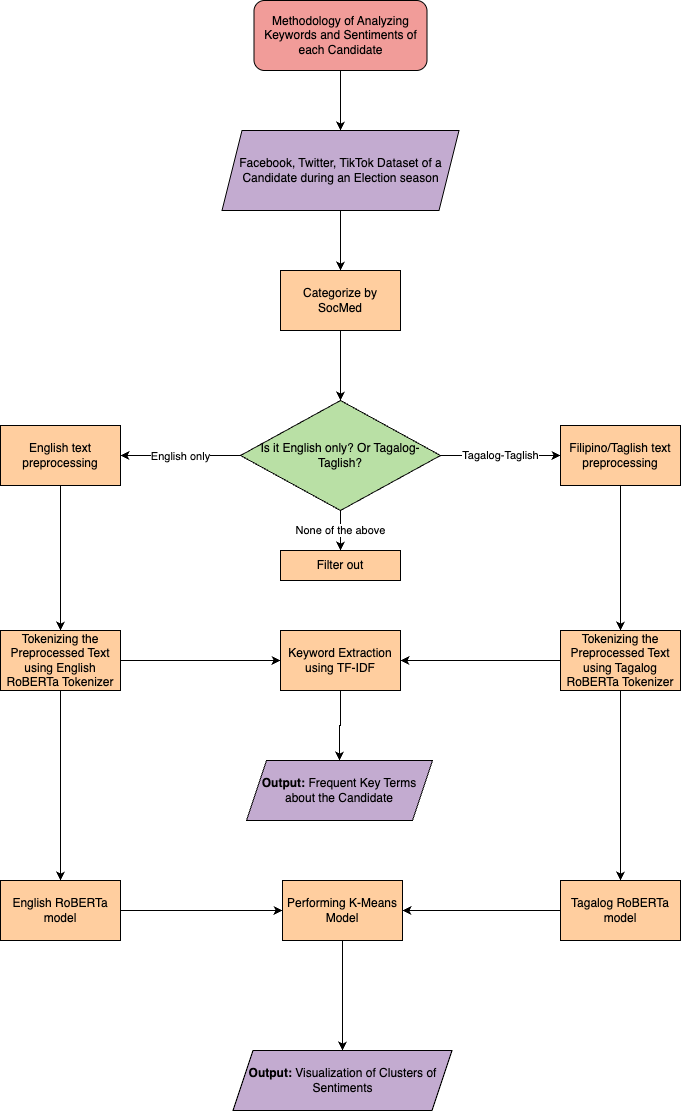
\includegraphics[width=1\textwidth]{Figures/methodology_flowchart.png}
    \caption{Methodology Flowchart}
    \label{fig:Methodology}
\end{figure}

% \clearpage

\section{Data Collection}
There are publicly available datasets for the 2024 US Presidential elections; however, for the 2022 Philippine Presidential Elections, the researchers will have to use a third-party Application Program Interface (API) due to the discontinued official free Academic API from X (former Twitter). In collecting tweets, keywords and dates will be utilized to perform an advanced search to get the tweets needed for the analysis.\newline

\begin{table}[h]
    \centering
    \begin{tabularx}{\textwidth}{X|X|X|X}
        \textbf{Presidential Election Year} & \textbf{Intention to Run Announcement} & \textbf{Dates within the Dataset (Inclusive)} & \textbf{Key Terms}\\
        \hline\hline
        \multirow{2}{*}{2022}& Marcos and Duterte: October 5, 2021 & \multirow{2}{*}{May 9, 2022} & \multirow{2}{4cm}{Marcos, Duterte, Robredo, Kiko, Pangilinan, BBM, Leni, DU30, Uniteam, Bongbong} \\
        & Robredo and Pangilinan: October 7, 2021 & & \\
    \end{tabularx}
    \caption{Table for Philippine Dataset Ranges}
\end{table}

\begin{table}[h]
    \centering
    \begin{tabularx}{\textwidth}{X|X|X|X}
        \textbf{Presidential Election Year} & \textbf{Intention to Run Announcement} & \textbf{Dates within the Dataset (Inclusive)} & \textbf{Key Terms}\\
        \hline\hline
        \multirow{2}{*}{2024}& Trump and Vance: November 15, 2022 & \multirow{2}{*}{November 8, 2024} & \multirow{2}{4cm}{Harris, Walz, Trump, Vance, Kamala, JD Vance} \\
        & Harris and Walz: July 21, 2024 & & \\
    \end{tabularx}
    \caption{Table for United States Dataset Ranges}
\end{table}

The end dates are until election day because of the high chances of a spike of sentiments especially as election days come closer.

Each collected tweet is in JSON format. For it to be utilized for natural language processing, it will be saved as a \texttt{.csv} file, separated, with each row marked by which country it belongs to, because it will be utilized for text classification.

\section{Data Preprocessing}
Before a group of datasets is fed into a tokenizer, they will undergo text processing.  Stop words such as \emph{“the,” “a,” “is”}, etc., will not be removed as they might be considered for the full context of a sentence when performing byte-tokenization. The following steps to preprocess the text will be as follows:

\begin{itemize}
    \item Omitting a tweet from the dataset if it is not in English, Tagalog, or a mix of them. The languages of the tweets will be detected by the Python library \texttt{langdetect}.
    \item Removing punctuation marks that have no significance for sentiment analysis.
    \item Replacing emojis with special tags.
    \item Removing unnecessary emojis or replacing emojis with special tags describing them if it is necessary for sentiment analysis.
    \item Lowercasing the text.
    \item Handling links and email addresses by replacing them with a placeholder.
    \item Removing whitespaces and replacing multiple spaces with a single space.
    \item Adding paddings to equalize the length of sentences.
\end{itemize}

The preprocessed dataset will be placed in a new \texttt{.csv} file. It is expected that the dataset, after they are preprocessed, will be 20,000 tweets per election.

\section{Text Classification and Visualization}
\subsection{XLM-RoBERTa}
After the preprocessing, the dataset will be fed into the following models: the \texttt{XLM-RoBERTa} model for contextualized embedding and the TF-IDF model for determining frequent keywords. XLM-RoBERTa’s language-agnostic approach makes it easier to implement as there is no need to identify if certain texts are in English or Tagalog.

Once the preprocessed dataset is fed into the model, the resulting tokens will be used to determine frequent keywords via TF-IDF and semantic similarities on the embedding model.

\subsection{GMM Model}
Once the embeddings are generated, they will be compared for semantic similarity via \texttt{Gausian Mixture Model (GMM)}, an unsupervised probabilistic clustering algorithm. GMM clustering, in contrast with K-Means clustering, are modelled as Gausian distributions, providing them flexbilitiy in handling overlapping clusters and variance differences, especially XLM-RoBERTa produces contextualized embeddings in high dimensions. In the context of nuanced tweets or tweets with mixed emotions, GMM’s soft clustering handles it better because it gives probability distributions, which is valuable for interpreting such tweets. The embeddings will be fed into the GMM model and it will provide soft assignments to each embedding, allowing them to belong to multiple clusters with different probabilities. The manually marked sentiments, which will be colored in the visualization, will serve as an evaluation to see if the tweets of same sentiments belong to the same clusters.

The clusters will be quantitatively evaluated by \texttt{Adjusted Rand Index\\(ARI)}, which examines the similarity between two clustering assignments. It will be used to determine if the agreement between the sentiment clusters and manually labelled sentiments.

% \subsection{K-Means Model}
% Once the embeddings are generated, they will be compared for semantic similarity via K-Means clustering. Since the model has a feature that helps determine if a tweet’s sentiment is positive, negative, or neutral, it will become a color indicator in the visualization of clusters to determine a cluster’s sentiment and visualize echo chambers. This will be crucial in comparing and contrasting the social media presence and activity of each candidate.

\subsection{TF-IDF}
Meanwhile, the tokenized texts will also go to the \texttt{TF-IDF model} to determine the frequency of words. The frequency of the words is sorted by how frequently they are used in a certain post or comment. The top keywords per candidate will be used to compare and contrast with other candidates and the social media spheres of the two countries.

\subsection{Visualization}
The interactive visualizations of the analysis consist of the following: a word cloud of the most frequent words and cluster visualization of semantic meanings. Using the time and date indicated in the dataset, they will be used to visualize the sentiments of the tweets during early election, mid-election, days before the election, and the election day itself. It will also highlight the surveys from public opinion polls to match if these strong sentiments has a correlation with the public polls and the election turnout on the day of election.
\begin{figure}[h]
    \centering
    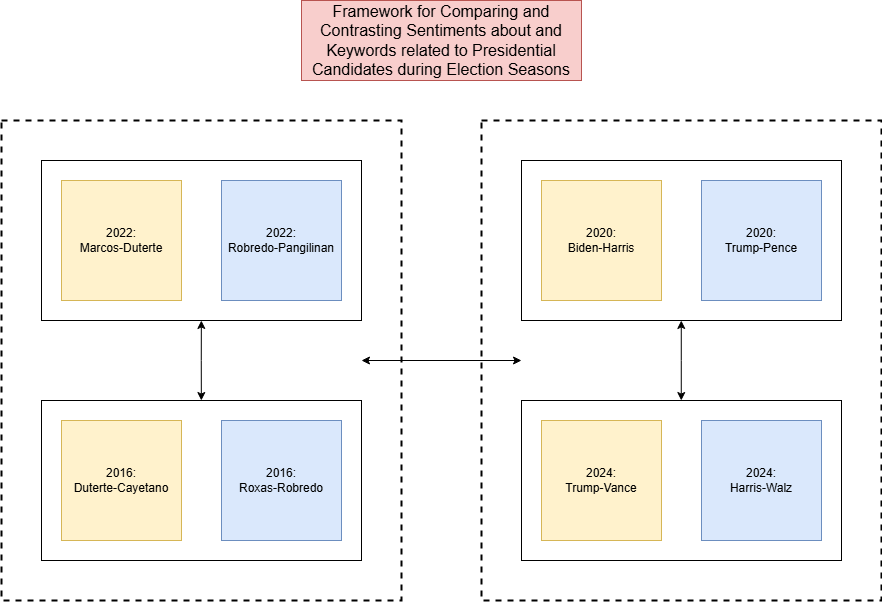
\includegraphics[width=0.65\textwidth]{Figures/methodology_framework-for-comparing.png}
    \caption{Framework for Comparing and Contrasting Sentiments}
    \label{fig:Framework-for-sentiments}
\end{figure}